%&tex

\chapter{Real world}\label{chp:realworld}

In this chapter we finally apply our model to a real-world implementation of mobile robot lane
following. We give reasons as to why we chose the models and pre-processing used in our real-world
experiment. Next, we describe how each model performed in each track. A video demonstration of the
robots in action is available online\footnote{\url{https://youtu.be/vhpWQDX2cQU}}. Finally, we give
some brief comments on the performance of the robots in general.

\section{Control and inference}

Our main goal in this project was to be able to provide a fast, accurate and robust model for
self-driving that was capable of real-time measurement of uncertainty. Emphasis must be placed on
real-time, as a self-driving car ought to react at least as fast as a human. For this reason, we
chose to use a very simple control system that relied on fast and accurate inference to perform
well.

In~\cite{self-driving}, the robot's control system employed a command queue. In their
implementation, the robot does not move itself until it receives a command. Once it does, it then
moves a fixed distance. If the next command is not ready to be processed, it stops and waits
for inference (i.e. the next command). Otherwise, the queued command is executed. These steps are
then repeated. Although this method of self-driving evaluation nicely quantifies accuracy, it fails
to account for inference speed.  Indeed, Moraes and Salvatore achieved $\approx$80\% accuracy with
deep feedforward neural networks and $\approx$85\% with convolutional neural networks, but
inference took about 1.35 seconds, with binarized results taking faster average speeds of 0.6
seconds, even with GPU support. In the real-world, a self-driving car cannot afford to run a few
meters, stop for inference, and then continue for a few more. We account for this in our
implementation.

For this reason, a much more reactive control system was built for this project. Input was based
solely on commands given by an inference model. Not only that, the speed of which these commands
were given impacted heavily on its performance. As mentioned in~\Cref{chp:hardware}, the Brick
receives a command and applies power to its motors accordingly. Until another command is given by
the Berry, the Brick repeats the same command previously given. For instance, if the Brick is given
a command to go straight, it will continue to do so without stopping until a different order is
otherwise given. This sort of control is able to quantify how reliable inference is based not only
on accuracy, but also speed of inference.

In~\Cref{chp:benchmarks}, we showed inference speed results based on a desktop computer with a
powerful CPU. When running the same models on the Berry, we found that although the binarized GD
architecture achieved 85\% accuracy and took about 0.3 seconds on a desktop PC, this speed went up
to 3.5 seconds on the Berry. This high increase is not only due to the power difference between the
two CPUs, but also by the need of real-time image pre-processing (in this case binarization)
directly from a live video feed.

This speed discrepancy forced us to discard several models due to slow inference. In fact, we found
that a model that took more than 0.15 seconds would take more than 1.0 second on the Berry.
Additionally, histogram equalization proved to severely decrease speeds, causing us to discard any
of its use in our real-world experimentations. We ultimately decided to use

\begin{enumerate}
  \item\label{item:setup-1} $Q_4$ and GD+d;
  \item\label{item:setup-2} $Q_6$ and GD+d;
  \item\label{item:setup-3} no pre-processing and GD+d.
\end{enumerate}

Inference times were about 0.7, 0.150 and 0.075 seconds for~\autoref{item:setup-1},
\autoref{item:setup-2} and \autoref{item:setup-3} respectively. All our implementations used solely
the CPU, with no GPU support. Our experiments show that a high accuracy but slow inference speed
performs poorly on our setup. A low accuracy but fast prediction speed model can behave
erratically, but is able to correct itself because of its speed. We found that a good balance
between accuracy and speed performed the best. We will refer as Model 1, Model 2 and Model 3 the
model and pre-processing done in~\autoref{item:setup-1}, \autoref{item:setup-2} and
\autoref{item:setup-3} respectively.

\section{Tracks}

We built three different tracks in order to evaluate how well models behaved in different
environments.  We assembled tracks in the same way as done in~\cite{self-driving}. In each track,
A4 paper sheets were placed in order to form road markings on both sides of the ``road''. In this
section, we describe each track and discuss how each model performed.

\subsection{Track 0}

The first track is a standard square shaped track. It is the simplest track we built in order to
evaluate turns and lines. The robot's objective is to complete a lap without going out of bounds.

\begin{figure}[h]
  \centering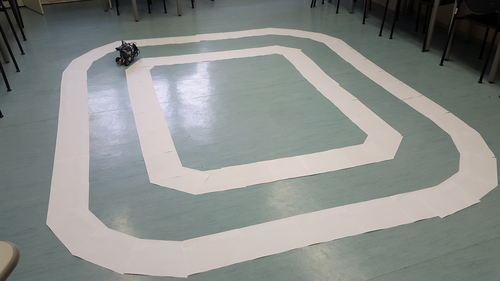
\includegraphics[width=0.9\textwidth]{imgs/track_0.png}
  \caption{Track 0 is a simple square shaped circuit.}
\end{figure}

All models were able to drive through the whole lap. We noticed that Model 1 was much slower in
terms of updating its state when compared to the other models. It particularly had trouble with
straight lines, as the model's slow inference speed prevented it from making small corrections and
thus propagated a sort of accumulated error at each attempted correction. Model 3 seemed to avoid
moving in a straight line, opting to zig-zag instead. This model's behavior was a constant in every
track. Model 2 was able to correctly turn and run lines with no apparent issue. Small corrections
when travelling on straight lines were handled well, as its fast inference speed allowed for fine
modifications to its direction.

\subsection{Track 1}

In this $\infty$-shaped track, the robot is supposed to travel through both conjoined circles,
alternating between the two of them without going out of bounds.

\begin{figure}[h]
  \centering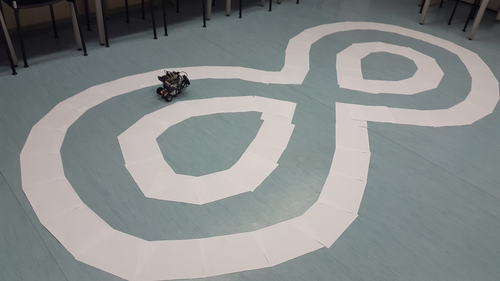
\includegraphics[width=0.9\textwidth]{imgs/track_1.png}
  \caption{Track 1 is an infinity shaped circuit.}
\end{figure}

Model 1 was unable to complete the lap, as once on the intersection of the two circles, the robot
kept its turning course, repeating the same circle instead of the other. This is due to its
slowness in updating its prediction, as the intersection point between the two circles could be
predicted as both a turn to the left, right or, as intended, a go straight command. All other
models were able to complete the two circles.

Model 2 completed the track perfectly, having no issue with traversing the intersection point.
Model 3 zig-zagged throughout the whole course, but was able to complete the track as well.

\subsection{Track 2}

The hardest of the tracks, it features sharp turns and irregular paths. One may map this artificial
scenario to the real-world challenge of roads in steep terrains, such as going down a mountain. An
additional challenge in this circuit is the proximity and otherwise intersection between road
markings that do not belong to the track the robot is currently on. This confuses the robot, as
depending on its position relative to the marks, it may incorrectly predict its next action.
Indeed, all models failed in this track directly or indirectly due to this.

\begin{figure}[h]
  \centering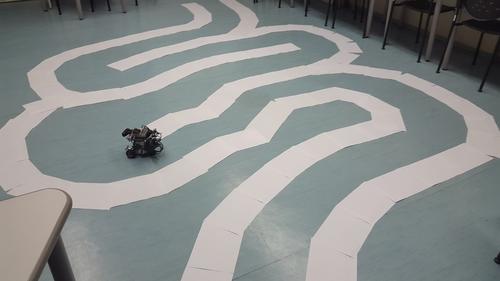
\includegraphics[width=0.9\textwidth]{imgs/track_2.png}
  \caption{Track 2 simulates a road going down a mountain.}
\end{figure}

Turns are identified by their order of appearance when travelling the pathway. Turns are
increasingly tighter as the road progresses. \autoref{fig:track-2-marks} marks these four turns
with visual aids colored in blue. We do the same for the three ambiguous road markings, coloring
them with red.

\begin{figure}[h]
  \centering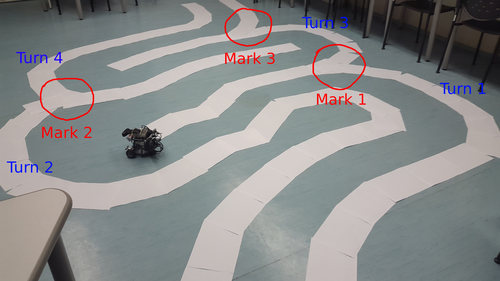
\includegraphics[width=0.9\textwidth]{imgs/track_2_marks.png}
  \caption{Track 2 ambiguous markings and sharp turns.\label{fig:track-2-marks}}
\end{figure}

Model 1 failed due to both ambiguous road markings (particularly on Mark 1) and the first sharp
turn (Turn 1). Because of its slow inference, it was unable to correct itself. Model 2 managed to
go all the way down to Turn 3, however it got confused on Mark 3, mistaking it for a right turn.
Model 3 failed on Mark 2 due to the same reasons.

Track 2 was designed with the flaws of our system in mind. We knew beforehand our approach with
image classification does not take into account previous classifications. This causes ambiguous
markings to be misclassified when they could have been inferred from previous predictions.
Likewise, sharp turns prove to be a challenge for a robot that is only allowed to go forward, as
one misclassification may prove fatal. Nevertheless, Model 2 exceeded our expectations, managing to
correctly travel through Turn 1 and Turn 2, and correctly evading Mark 1 and Mark 2.

\section{Comments}

Although our experiments have shown that image classification for self-driving is not perfect, it
is worthy to mention that the robots were able to correctly extrapolate from data. Even though the
materials used to build the tracks were identical to the dataset's, the tracks themselves were very
distinct from what was used in the original's. This shows how SPNs were able to generalize from
their training data. Model 2 especially was able to correctly classify both Marks 1 and 2 despite
never seeing this kind of road marking in its training dataset. It is also worthy to mention that,
although Model 3 failed to go straight when presented with a straight line, the probabilities
computed by the model to go UP when on a line were very often high, meaning the model had some
sense of uncertainty between turning and going straight.

We also noticed that calibration seemed to have played a major role in how well the models
performed.  In fact, the correct positioning of the camera, i.e. its angle with relation to the
ground and its height, was crucial for making the robot work. Self-driving image classification
seems to be very sensitive with respect to this. The training dataset had a specific camera angle
and height that we attempted to replicate as best as possible. In spite of this, as the robot is in
constant movement, and because of small vibrations made by the Brick's motors, the camera angle was
often disturbed, causing the robot to misclassify. However this could easily be solved by affixing
the camera to the robot itself.

Another recurring issue we had were CPU processing interruptions. Often, the Raspberry Pi would
completely halt the program's runtime.  We are unsure if this was an OS interruption or if it was
related to the power source, as we were using several periphericals for input and output whilst
using an underpowered battery source. This can be viewed in the demonstration video, where Model
2's front video feed in Track 0 skips several frames during recording.

Overall, the models were able to perform fairly well, although with some minor technical issues.
